
\subsection{Answers}
\begin{table}[htb]%
\begin{center}%
\caption{Q4: What programming language(s) do you use most often?}%
\label{tab:Q4-ans}%
\begin{tabular}{l|l|r}%
\hline%
Choice & Abbrv. & \# Answers \\%
\hline%
C/C++ & C(++) & 665 (78.2\%) \\%
Python & Py & 433 (50.9\%) \\%
Fortran 90 or newer & \verb!>!=F90 & 373 (43.9\%) \\%
Fortran (older one than Fortran 90) & \verb!<!F90 & 139 (16.4\%) \\%
Java & Java & 47 (5.5\%) \\%
other & - & 70 (8.2\%) \\%
\hline%
\multicolumn{2}{c}{total} & 1727 (850)\\%
\hline%
\end{tabular}%
\end{center}%
\end{table}%

\clearpage%
{\footnotesize\begin{landscape}%
\begin{longtable}[htb]{r|c|c|c|c|c|c|c|c|c|c}%
\caption{Q4: What programming language(s) do you use most often?}%
\label{tab:Q4-mans} \\%
\hline%
Multi-Answer & overall & FR & GR & IT & UK & eu & JP & RU & US & others \\
 \hline%
\endfirsthead%
\multicolumn{11}{r}{(continued from the previous page)}\\%
\hline%
Multi-Answer & overall & FR & GR & IT & UK & eu & JP & RU & US & others \\
 \hline%
\endhead%
\hline%
(total) & 850 & 125 & 159 & 57 & 67 & 144 & 64 & 94 & 58 & 82 \\%
\hline%
\multicolumn{11}{r}{(continue to the next page)}\\%
\endfoot%
\hline%
(total) & 850 & 125 & 159 & 57 & 67 & 144 & 64 & 94 & 58 & 82 \\%
\hline%
\endlastfoot%
\hline%
{C(++), Py} & 178 & 25 & 44 & 8 & 7 & 31 & 12 & 27 & 7 & 17 \\%
{C(++)} & 175 & 23 & 29 & 12 & 10 & 25 & 18 & 24 & 14 & 20 \\%
{C(++), \verb!>!=F90, Py} & 90 & 19 & 15 & 7 & 12 & 20 & 6 & 2 & 6 & 3 \\%
{C(++), \verb!>!=F90} & 61 & 8 & 12 & 4 & 4 & 13 & 6 & 4 & 2 & 8 \\%
{\verb!>!=F90} & 56 & 13 & 13 & 5 & 5 & 7 & 3 & 3 & 2 & 5 \\%
{\verb!>!=F90, Py} & 39 & 6 & 8 & 4 & 5 & 11 & 1 & 0 & 2 & 2 \\%
{C(++), \verb!<!F90, \verb!>!=F90} & 33 & 5 & 5 & 1 & 2 & 2 & 3 & 9 & 6 & 0 \\%
{C(++), \verb!<!F90, \verb!>!=F90, Py} & 23 & 2 & 4 & 3 & 1 & 4 & 2 & 0 & 2 & 5 \\%
{\verb!<!F90, \verb!>!=F90} & 19 & 2 & 3 & 2 & 1 & 2 & 3 & 2 & 1 & 3 \\%
{\verb!<!F90, \verb!>!=F90, Py} & 17 & 3 & 4 & 0 & 1 & 4 & 0 & 4 & 0 & 1 \\%
{C(++), Java, Py} & 15 & 2 & 2 & 0 & 1 & 1 & 3 & 3 & 1 & 2 \\%
{Py} & 14 & 1 & 1 & 4 & 1 & 5 & 0 & 0 & 0 & 2 \\%
{C(++), \verb!<!F90, Py} & 11 & 3 & 4 & 1 & 0 & 1 & 0 & 1 & 1 & 0 \\%
{C(++), \verb!<!F90} & 11 & 1 & 1 & 2 & 1 & 0 & 2 & 2 & 1 & 1 \\%
{\verb!<!F90} & 10 & 1 & 1 & 0 & 1 & 2 & 1 & 0 & 1 & 3 \\%
{C(++), \verb!<!F90, \verb!>!=F90, Java} & 8 & 0 & 0 & 0 & 8 & 0 & 0 & 0 & 0 & 0 \\%
{C(++), Java} & 8 & 1 & 1 & 0 & 0 & 1 & 0 & 3 & 0 & 2 \\%
{C(++), Julia} & 4 & 0 & 1 & 0 & 0 & 0 & 0 & 1 & 2 & 0 \\%
{Java, Py} & 4 & 1 & 0 & 1 & 0 & 0 & 0 & 0 & 0 & 2 \\%
{Julia} & 3 & 0 & 0 & 0 & 0 & 1 & 0 & 0 & 2 & 0 \\%
{C(++), \verb!>!=F90, Java, Py} & 3 & 1 & 0 & 0 & 1 & 0 & 0 & 1 & 0 & 0 \\%
{C(++), Perl} & 2 & 2 & 0 & 0 & 0 & 0 & 0 & 0 & 0 & 0 \\%
{\verb!>!=F90, Julia} & 2 & 0 & 1 & 0 & 0 & 1 & 0 & 0 & 0 & 0 \\%
{Java} & 2 & 0 & 0 & 0 & 0 & 1 & 0 & 1 & 0 & 0 \\%
{C(++), Py, Shell} & 2 & 1 & 0 & 0 & 0 & 0 & 0 & 0 & 1 & 0 \\%
{C(++), Py, CUDA} & 2 & 0 & 0 & 1 & 0 & 0 & 0 & 1 & 0 & 0 \\%
{\verb!>!=F90, Py, Julia} & 2 & 0 & 1 & 1 & 0 & 0 & 0 & 0 & 0 & 0 \\%
{C(++), \verb!>!=F90, Py, Matlab} & 2 & 0 & 1 & 0 & 1 & 0 & 0 & 0 & 0 & 0 \\%
{R} & 1 & 1 & 0 & 0 & 0 & 0 & 0 & 0 & 0 & 0 \\%
{Py, Perl} & 1 & 0 & 1 & 0 & 0 & 0 & 0 & 0 & 0 & 0 \\%
{C(++), Py, R, Javascript} & 1 & 0 & 0 & 0 & 0 & 0 & 0 & 0 & 1 & 0 \\%
{\verb!>!=F90, Py, bash} & 1 & 0 & 0 & 0 & 1 & 0 & 0 & 0 & 0 & 0 \\%
{C(++), \verb!<!F90, C\#} & 1 & 0 & 0 & 0 & 0 & 0 & 0 & 0 & 0 & 1 \\%
{\verb!>!=F90, Py, ncl} & 1 & 0 & 0 & 0 & 0 & 0 & 0 & 1 & 0 & 0 \\%
{C(++), D, C\#} & 1 & 0 & 0 & 0 & 0 & 0 & 0 & 1 & 0 & 0 \\%
{C(++), \verb!>!=F90, Shell scripts, Perl} & 1 & 0 & 0 & 0 & 1 & 0 & 0 & 0 & 0 & 0 \\%
{C(++), \verb!>!=F90, Perl} & 1 & 0 & 0 & 0 & 1 & 0 & 0 & 0 & 0 & 0 \\%
{C(++), Py, BASH, Perl} & 1 & 0 & 0 & 0 & 0 & 0 & 0 & 0 & 1 & 0 \\%
{\verb!>!=F90, Matlab} & 1 & 0 & 0 & 1 & 0 & 0 & 0 & 0 & 0 & 0 \\%
{C(++), \verb!<!F90, \verb!>!=F90, Java, C\# VB} & 1 & 0 & 0 & 0 & 0 & 0 & 0 & 0 & 0 & 1 \\%
{C(++), Py, haskell, matlab, wolfram mathematica} & 1 & 0 & 0 & 0 & 0 & 0 & 0 & 1 & 0 & 0 \\%
{C(++), Py, Common Lisp} & 1 & 0 & 0 & 0 & 0 & 1 & 0 & 0 & 0 & 0 \\%
{C(++), Bash, sed, Makefile, TeX} & 1 & 0 & 1 & 0 & 0 & 0 & 0 & 0 & 0 & 0 \\%
{C(++), Rust} & 1 & 0 & 0 & 0 & 0 & 1 & 0 & 0 & 0 & 0 \\%
{C(++), \verb!>!=F90, Py, C\#} & 1 & 0 & 0 & 0 & 0 & 1 & 0 & 0 & 0 & 0 \\%
{Py, Julia} & 1 & 0 & 0 & 0 & 0 & 0 & 0 & 0 & 1 & 0 \\%
{C(++), bash, R} & 1 & 0 & 0 & 0 & 1 & 0 & 0 & 0 & 0 & 0 \\%
{C(++), \verb!>!=F90, julia} & 1 & 1 & 0 & 0 & 0 & 0 & 0 & 0 & 0 & 0 \\%
{C(++), Py, Go} & 1 & 0 & 0 & 0 & 0 & 1 & 0 & 0 & 0 & 0 \\%
{Java, Py, R, Perl} & 1 & 0 & 0 & 0 & 0 & 1 & 0 & 0 & 0 & 0 \\%
{C(++), Py, R} & 1 & 0 & 0 & 0 & 0 & 1 & 0 & 0 & 0 & 0 \\%
{\verb!>!=F90, Py, Guile Scheme, R} & 1 & 0 & 0 & 0 & 0 & 1 & 0 & 0 & 0 & 0 \\%
{\verb!<!F90, Py} & 1 & 0 & 1 & 0 & 0 & 0 & 0 & 0 & 0 & 0 \\%
{\verb!<!F90, \verb!>!=F90, Perl5 IDL} & 1 & 0 & 1 & 0 & 0 & 0 & 0 & 0 & 0 & 0 \\%
{C(++), \verb!>!=F90, Py, matlab} & 1 & 1 & 0 & 0 & 0 & 0 & 0 & 0 & 0 & 0 \\%
{\verb!>!=F90, Java, Py} & 1 & 0 & 0 & 0 & 0 & 0 & 0 & 0 & 1 & 0 \\%
{\verb!>!=F90, Ruby} & 1 & 0 & 0 & 0 & 0 & 0 & 1 & 0 & 0 & 0 \\%
{\verb!>!=F90, Py, js} & 1 & 1 & 0 & 0 & 0 & 0 & 0 & 0 & 0 & 0 \\%
{C(++), Py, bash} & 1 & 0 & 1 & 0 & 0 & 0 & 0 & 0 & 0 & 0 \\%
{C(++), Java, Py, Perl} & 1 & 0 & 0 & 0 & 1 & 0 & 0 & 0 & 0 & 0 \\%
{C(++), UPC} & 1 & 0 & 0 & 0 & 0 & 0 & 0 & 0 & 1 & 0 \\%
{C(++), CUDA, OpenCL} & 1 & 0 & 0 & 0 & 0 & 1 & 0 & 0 & 0 & 0 \\%
{C(++), Lisp, Ocaml, Perl} & 1 & 0 & 0 & 0 & 0 & 0 & 1 & 0 & 0 & 0 \\%
{\verb!>!=F90, Pascal/Delphi} & 1 & 0 & 0 & 0 & 0 & 0 & 0 & 1 & 0 & 0 \\%
{C(++), \verb!<!F90, \verb!>!=F90, Py, tcl/tk} & 1 & 0 & 1 & 0 & 0 & 0 & 0 & 0 & 0 & 0 \\%
{C(++), Java, Py, Rust} & 1 & 0 & 0 & 0 & 0 & 1 & 0 & 0 & 0 & 0 \\%
{Py, R} & 1 & 0 & 0 & 0 & 0 & 0 & 1 & 0 & 0 & 0 \\%
{Py, OCaml} & 1 & 0 & 0 & 0 & 0 & 0 & 0 & 0 & 1 & 0 \\%
{C(++), Py, Rust} & 1 & 0 & 0 & 0 & 0 & 1 & 0 & 0 & 0 & 0 \\%
{C(++), Py, JavaScript, MATLAB} & 1 & 0 & 0 & 0 & 0 & 0 & 1 & 0 & 0 & 0 \\%
{C(++), Py, Octave} & 1 & 0 & 0 & 0 & 0 & 1 & 0 & 0 & 0 & 0 \\%
{C(++), \verb!<!F90, \verb!>!=F90, Py, Julia} & 1 & 0 & 0 & 0 & 0 & 0 & 0 & 0 & 1 & 0 \\%
{C(++), \verb!<!F90, \verb!>!=F90, Java, Py} & 1 & 0 & 0 & 0 & 0 & 0 & 0 & 0 & 0 & 1 \\%
{C(++), Py, MATLAB script} & 1 & 0 & 0 & 0 & 0 & 0 & 0 & 0 & 0 & 1 \\%
{C(++), Ruby} & 1 & 0 & 0 & 0 & 0 & 1 & 0 & 0 & 0 & 0 \\%
{C(++), Java, MATLAB} & 1 & 0 & 0 & 0 & 0 & 0 & 0 & 0 & 0 & 1 \\%
{C(++), JavaScript} & 1 & 0 & 0 & 0 & 0 & 0 & 0 & 1 & 0 & 0 \\%
{Py, bash?} & 1 & 0 & 0 & 0 & 0 & 0 & 0 & 0 & 0 & 1 \\%
{C(++), Matlab} & 1 & 0 & 1 & 0 & 0 & 0 & 0 & 0 & 0 & 0 \\%
{C(++), Bash, Lua, Ruby} & 1 & 0 & 0 & 0 & 0 & 0 & 0 & 1 & 0 & 0 \\%
{C(++), C\# (through c bindings)} & 1 & 1 & 0 & 0 & 0 & 0 & 0 & 0 & 0 & 0 \\%
{C(++), Py, bash, awk, rust} & 1 & 0 & 1 & 0 & 0 & 0 & 0 & 0 & 0 & 0 \\%
\hline%
\end{longtable}%
\end{landscape}}%
\clearpage%


Although C/C++ was the most widely used programming language by the
respondents,  
it turns out that Python and Fortran are used similarly.  The use of
Python is 
also a strong indication Python binding for MPI could also be strongly
considered. There were no
country-to-country variations, and all regions had similar ratios.

\subsection{List of other answers}
\begin{itemize}
\item Asia: C\# VB
\item Central and South America: C\#
\item Central and South America: bash?
\item Europe:France: C\# (through c bindings)
\item Europe:France: Perl
\item Europe:France: Perl
\item Europe:France: R
\item Europe:France: Shell
\item Europe:France: js
\item Europe:France: julia
\item Europe:France: matlab
\item Europe:Germany: Bash, sed, Makefile, TeX
\item Europe:Germany: Julia
\item Europe:Germany: Julia
\item Europe:Germany: Julia
\item Europe:Germany: Matlab
\item Europe:Germany: Matlab
\item Europe:Germany: Perl
\item Europe:Germany: Perl5 IDL
\item Europe:Germany: bash
\item Europe:Germany: bash, awk, rust
\item Europe:Germany: tcl/tk
\item Europe:Italy: CUDA
\item Europe:Italy: Julia
\item Europe:Italy: Matlab
\item Europe:UK: Matlab
\item Europe:UK: Perl
\item Europe:UK: Perl
\item Europe:UK: Shell scripts, Perl
\item Europe:UK: bash
\item Europe:UK: bash, R
\item Europe:others: C\#
\item Europe:others: CUDA, OpenCL
\item Europe:others: Common Lisp
\item Europe:others: Go
\item Europe:others: Guile Scheme, R
\item Europe:others: Julia
\item Europe:others: Julia
\item Europe:others: Octave
\item Europe:others: R
\item Europe:others: R, Perl
\item Europe:others: Ruby
\item Europe:others: Rust
\item Europe:others: Rust
\item Europe:others: Rust
\item Japan: JavaScript, MATLAB
\item Japan: Lisp, Ocaml, Perl
\item Japan: R
\item Japan: Ruby
\item Russia: Bash, Lua, Ruby
\item Russia: CUDA
\item Russia: D, C\#
\item Russia: JavaScript
\item Russia: Julia
\item Russia: Pascal/Delphi
\item Russia: haskell, matlab, wolfram mathematica
\item Russia: ncl
\item South Korea: MATLAB
\item South Korea: MATLAB script
\item USA: BASH, Perl
\item USA: Julia
\item USA: Julia
\item USA: Julia
\item USA: Julia
\item USA: Julia
\item USA: Julia
\item USA: OCaml
\item USA: R, Javascript
\item USA: Shell
\item USA: UPC

\end{itemize}

\begin{figure}[htb]
\begin{center}
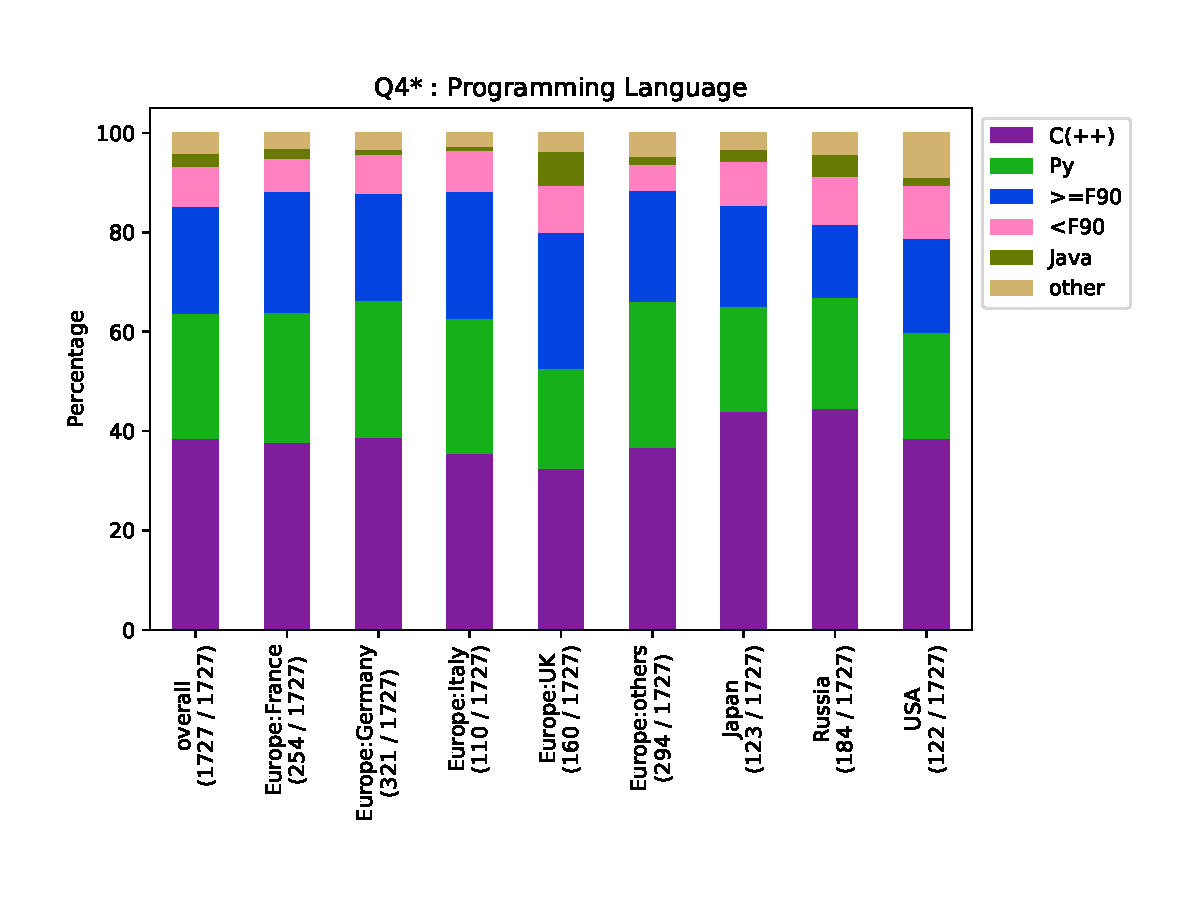
\includegraphics[width=10cm]{../pdfs/Q4.pdf}
\caption{Simple analysis: Q4}
\label{fig:Q4}
\end{center}
\end{figure}

\begin{figure}[htb]
\begin{center}
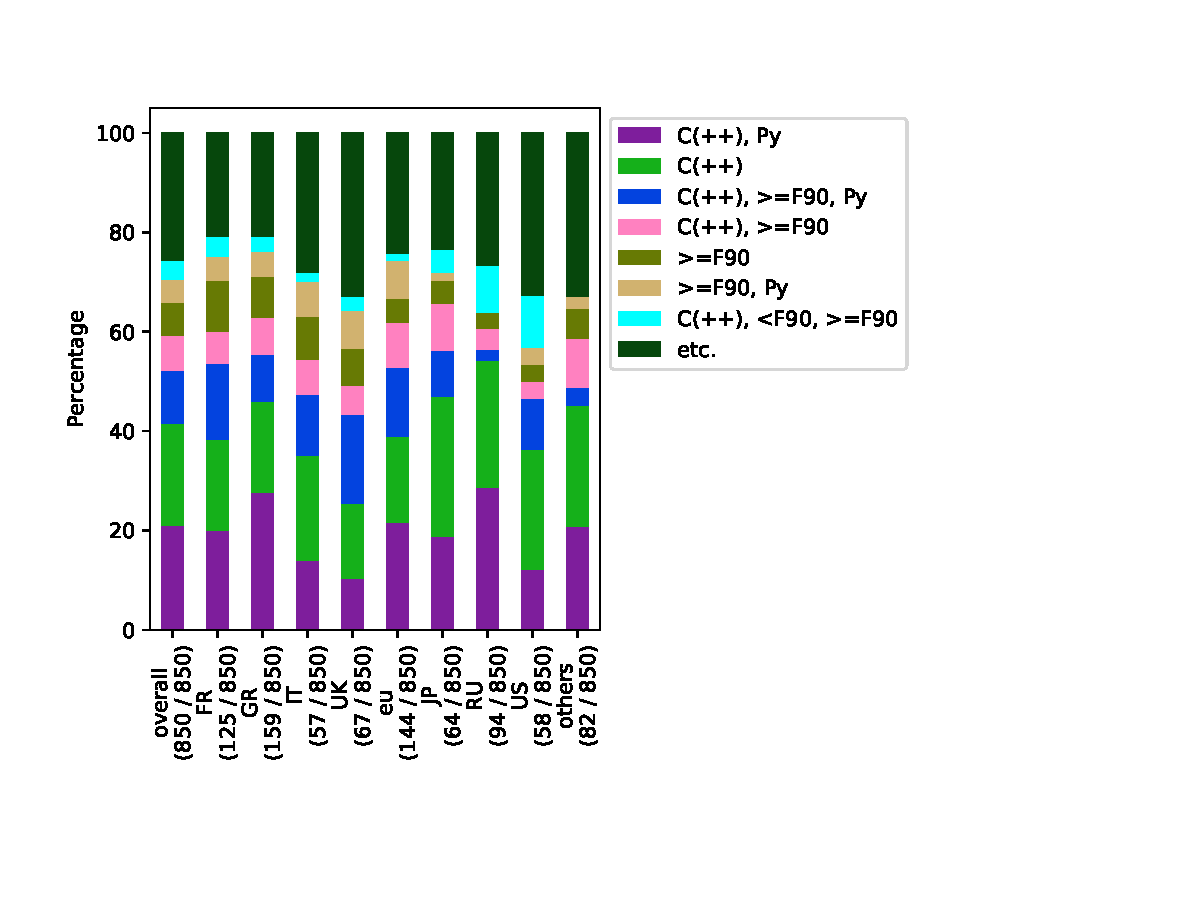
\includegraphics[width=14cm]{../pdfs/Q4-mans.pdf}
\caption{Multiple-Answers: Q4}
\label{fig:Q4-mans}
\end{center}
\end{figure}
